\documentclass[a4paper,12pt]{article}
\usepackage[utf8]{inputenc}
\usepackage[T1]{fontenc}
\usepackage[french]{babel}
\usepackage{amsmath}
\usepackage{amsfonts}
\usepackage{graphicx}
\usepackage{geometry}
\usepackage{titlesec}
\usepackage{tocloft}
\usepackage{caption}
\usepackage{array}
\usepackage{tikz}
\usepackage{pgfplots}
\usepackage{hyperref}
\usepackage{minted}
\usepackage{framed}
\usepackage{xcolor}
\usepackage{fancyhdr} % Pour personnaliser les en-têtes et pieds de page
\usepackage{float} % Pour utiliser [H]

\geometry{top=2.5cm, bottom=2.5cm, left=2cm, right=2.5cm}

% Formatage des titres
\titleformat{\section}{\large\bfseries}{\thesection}{1em}{}
\titleformat{\subsection}{\normalsize\bfseries}{\thesubsection}{1em}{}

% Configuration de hyperref
\hypersetup{
    pdfborder={0 0 0}       % Supprime les cadres autour des liens
}
% Configuration de la table des matières
\renewcommand{\cftsecfont}{\bfseries}
\renewcommand{\cftsecpagefont}{\bfseries}
\renewcommand{\cftsubsecfont}{\normalfont}
\renewcommand{\cftsubsecpagefont}{\normalfont}

% Configuration de l'en-tête
\fancypagestyle{custom}{%
    \fancyhf{} % Réinitialise les en-têtes et pieds de page
    \renewcommand{\headrulewidth}{0.4pt} % Définit la largeur de la ligne (1pt ici)
    \fancyhead[L]{SCAIA Matteo, GILLET Louison} % Texte dans l'en-tête gauche
    \fancyhead[R]{HAX907X-M2 MIND} % Numéro de page dans l'en-tête droite
     \fancyfoot[C]{\thepage} % Numéro de page centré dans le pied de page
}
\setlength{\parindent}{0pt}

\title{\textbf{HAX907X Support Vector Machine}}
\author{{SCAIA Matteo} \qquad {GILLET Louison}}
\date{2025-2026}

\begin{document}

\begin{titlepage}
    \centering
    \vspace*{\fill} % pousse le contenu vers le milieu

    \rule{\textwidth}{0.4pt}\\[1cm] % barre fine horizontale
    {\Huge \textbf{HAX907X Support Vector Machine}\par}
    \vspace{0.5cm}
    {\large SCAIA Matteo \qquad GILLET Louison \par}
    \vspace{0.5cm}
    {\large 2025--2026 \par}
    \rule{\textwidth}{0.4pt} % barre fine horizontale

    \vspace*{\fill} % espace après pour centrer verticalement

    % Logos en bas de page
    \begin{figure}[!b] 
        \centering
        
\includegraphics[width=0.2\textwidth]{images/logo_um.pdf} \hspace{1cm}
        
\includegraphics[width=0.2\textwidth]{images/Faculte-des-Sciences-2022-rond-fond.png} \hspace{1cm}
        
\includegraphics[width=0.2\textwidth]{images/ssd_logo_couleur_noir-300x103.png}
    \end{figure}
\end{titlepage}

\newpage
\tableofcontents
\vspace{2cm}
\listoffigures
\newpage

\pagestyle{custom}
\section{Classification de la classe 1 contre la classe 2}

Dans un premier temps, on évite que les données soient triées par classe en 
permutant aléatoirement les lignes de \texttt{X} et les valeurs correspondantes 
de \texttt{y}, grâce à l’option \texttt{shuffle=True}\footnote{Pour la reproductibilité, on fixe la graine à 42 : \texttt{random\_state=42}.} de la fonction 
\texttt{train\_test\_split}. L’ensemble est ensuite scindé en deux parties : 
un jeu d’apprentissage représentant 75\% des données et un jeu de test 
représentant les 25\% restants.

\begin{minted}[frame=single, linenos, fontsize=\small, breaklines]{python}
# split train test
X_train, X_test, y_train, y_test = train_test_split(X, y, test_size=0.25, random_state=42, shuffle=True)
\end{minted}

\subsection{Noyau linéaire}

En se basant sur les définitions et notations de l'énoncé, nous utilisons un noyau linéaire de la forme : 
\[ K(x, x') = \langle x, x' \rangle \]

\begin{minted}[frame=single, linenos, fontsize=\small, breaklines]{python}
parameters = {'kernel': ['linear'], 'C': list(np.logspace(-3, 3, 200))}
clf = SVC()
clf_linear = GridSearchCV(clf, parameters, n_jobs=-1)
clf_linear.fit(X_train, y_train)

# compute the score
print(clf_linear.best_params_)
print('Generalization score for linear kernel: %s, %s' %
      (clf_linear.score(X_train, y_train),
       clf_linear.score(X_test, y_test)))
\end{minted}

Nous obtenons la sortie suivante : 
\begin{minted}[frame=single, fontsize=\small, breaklines]
{'C': 0.8406652885618325, 'kernel': 'linear'}
Generalization score for linear kernel: 0.7466666666666667, 0.68
\end{minted}


Avec un SVM à noyau linéaire, le meilleur paramètre trouvé est $C\approx 0.074$. Cela montre que le modèle accepte plus facilement des erreurs sur les points mal classés afin de privilégier une frontière de décision plus souple.
Le modèle obtient un score d'apprentissage d'environ $0.75$. Ce résultat indique qu'il se trompe déjà sur près de $25$ \% des données d'entraînement. Sur l'ensemble de test, il obtient un score de $0.68$. Ces résultats traduisent une faible capacité de généralisation, le modèle ne parvient pas à bien dissocier les deux classes.\\

\subsection{Noyau polynomial}

On cherche à comparer ces résultats avec un SVM basé sur un noyau polynomial. Ce noyau est de la forme : 

\[K(x,x')=(\alpha + \beta\langle x,x'\rangle)^\delta \quad \text{pour un $\delta$ > 0}\]

\begin{minted}[frame=single, linenos, fontsize=\small, breaklines]{python}
Cs = list(np.logspace(-3, 3, 5))
gammas = 10. ** np.arange(1, 2)
degrees = np.r_[1, 2, 3]

parameters = {'kernel': ['poly'], 'C': Cs, 'gamma': gammas, 'degree': degrees}
clf = SVC()
clf_poly = GridSearchCV(clf, parameters, n_jobs=-1)
clf_poly.fit(X_train, y_train)

print(clf_poly.best_params_)
print('Generalization score for polynomial kernel: %s, %s' %
      (clf_poly.score(X_train, y_train),
       clf_poly.score(X_test, y_test)))
\end{minted}

Cette fois, nous obtenons les résultats suivants : 
\begin{minted}[frame=single, fontsize=\small, breaklines]
{'C': 0.03162277660168379, 'degree': 1, 'gamma': 10.0, 'kernel': 'poly'}
Generalization score for polynomial kernel: 0.7466666666666667, 0.68
\end{minted}

La validation croisée a retenu un polynôme de degré 1, ce qui correspond en réalité à un modèle linéaire. Cela explique le fait que les scores d'apprentissage et de test soient identiques au SVM à noyau linéaire.\\

Nous proposons finalement de visualiser graphiquement nos données afin de mieux comprendre leur répartition et les phénomènes observés.

\begin{figure}[H] 
    \centering
    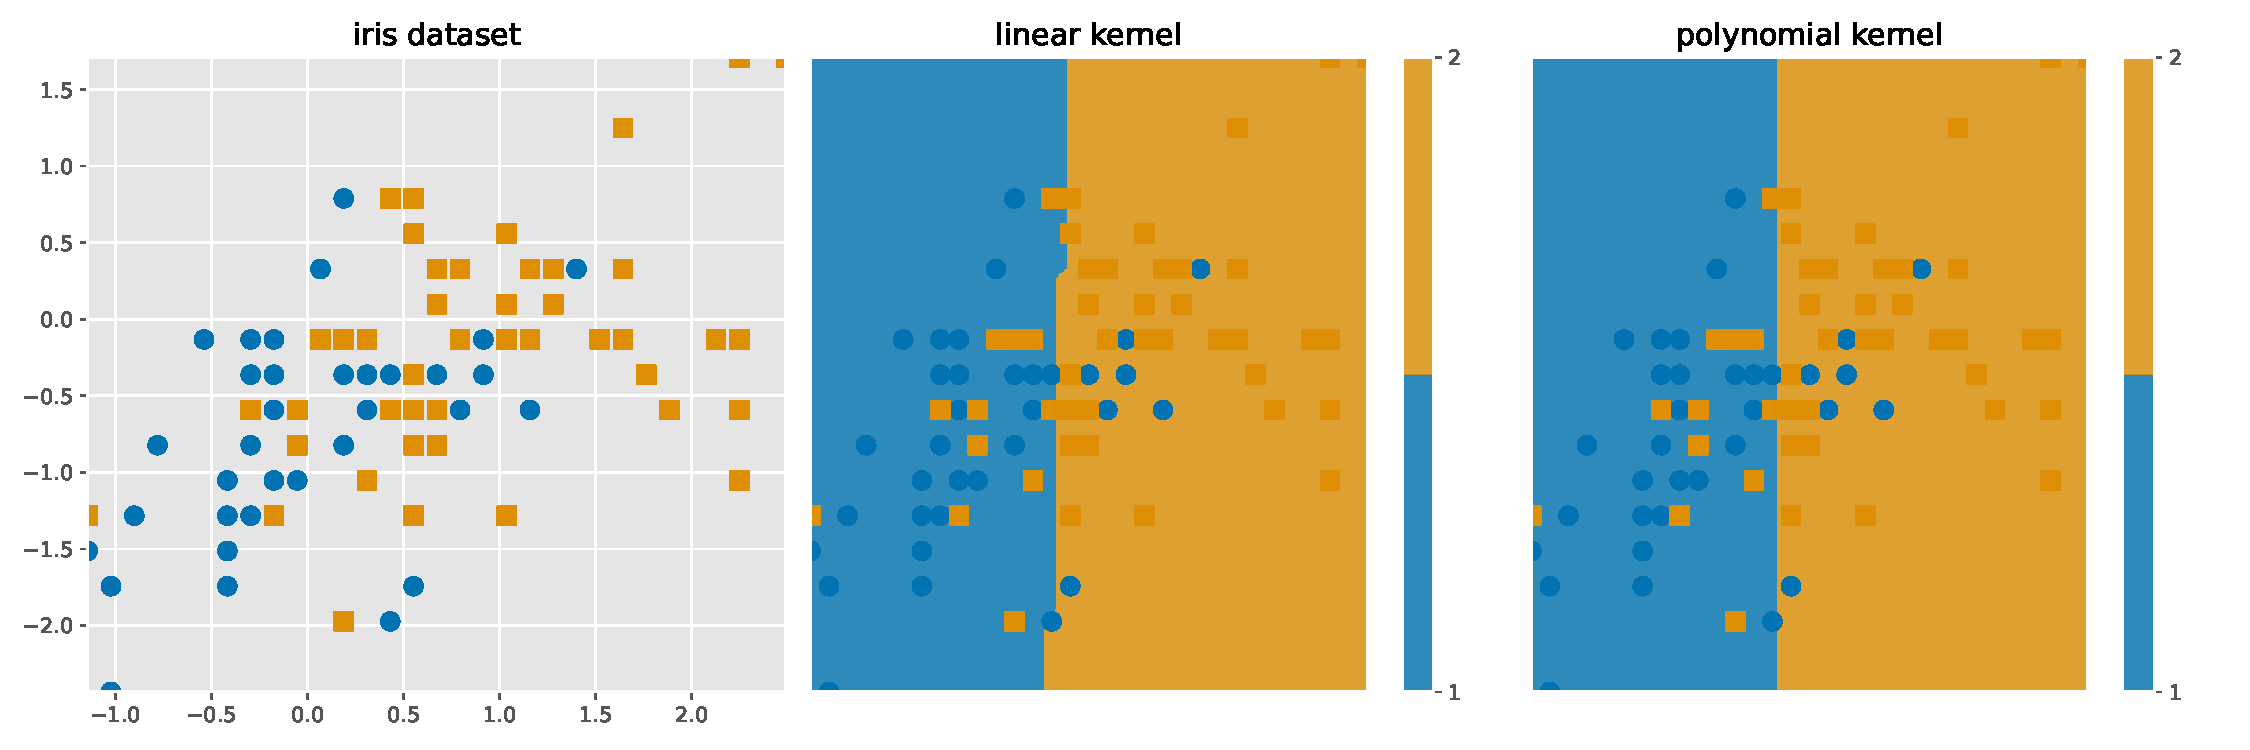
\includegraphics[width=\textwidth]{images/fig_iris.pdf} 
    \caption{Représentation du jeu de données Iris et classification par SVM à noyau linéaire et polynomial}
    \label{fig:iris_2D}
\end{figure}

On observe sur la figure \ref{fig:iris_2D} que de nombreux points des deux classes se chevauchent ce qui rend impossible une séparation nette par une frontière, qu'elle soit linéaire ou polynomiale. On retrouve ce problème dans les deux représentations où l'on voit que de nombreux points se retrouvent mal classifiés. 

En conclusion, ces résultats montrent que dans l’espace réduit aux deux premières variables, la classification des deux classes d’iris est difficile car elles ne sont pas linéairement séparables.

\subsection{Remarque}
Par ailleurs, pour mettre en évidence l’impact crucial du mélange initial des données, nous proposons d’analyser les performances du modèle en fixant l’option \texttt{shuffle=False} dans la fonction \texttt{train\_test\_split}. On obtient les scores suivants : 

\begin{minted}[frame=single, fontsize=\small, breaklines]
{'C': 0.3409285069746811, 'kernel': 'linear'}
Generalization score for linear kernel: 0.7466666666666667, 0.28
{'C': 0.001, 'degree': 2, 'gamma': 10.0, 'kernel': 'poly'}
Generalization score for polynomial kernel: 0.76, 0.2
\end{minted}

On observe que les scores d'apprentissage sont proches de ceux obtenus précédemment. En revanche, les scores de test chutent de manière drastique ce qui révéle une très mauvaise capacité de généralisation. Cela montre que lorsque les données ne sont pas mélangées, l’ensemble d’entraînement peut ne pas être représentatif de l’ensemble de test, et le modèle apprend alors des caractéristiques spécifiques aux données d'entraînement plutôt que des motifs généraux.\\


\section{SVM GUI}

On cherche à évaluer l’impact du choix du noyau et du paramètre C dans un SVM. Pour cela, on génère un jeu de données très déséquilibré de deux classes, qu'on représente sur la figure \ref{fig:plot_svm_gui}.

\begin{figure}[H] 
    \centering
    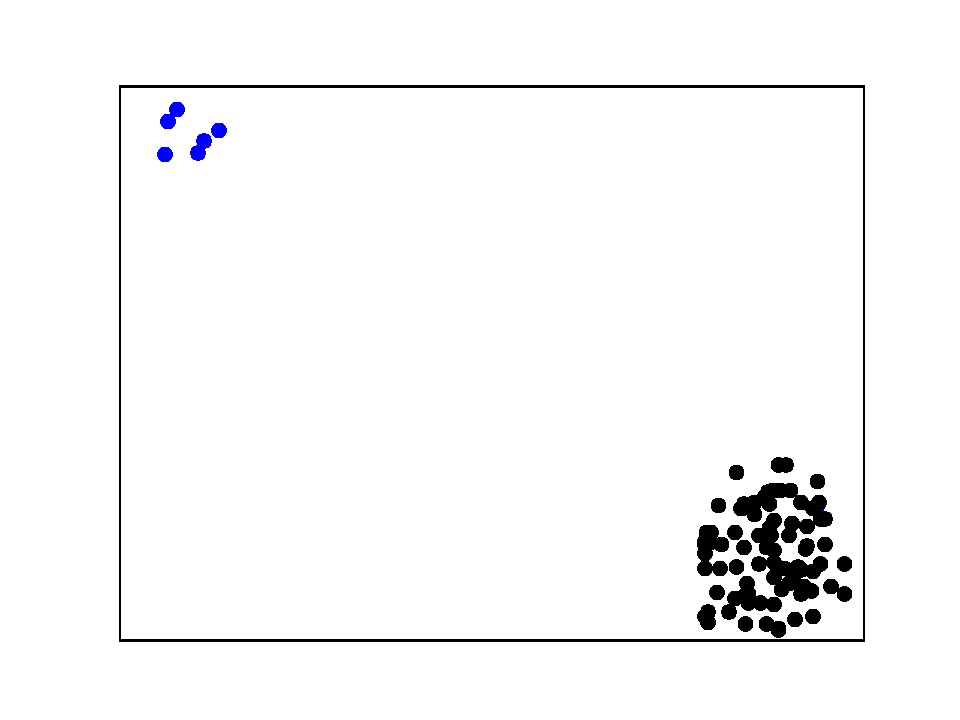
\includegraphics[width=0.7\textwidth]{images/plot.pdf} 
    \caption{Représensation d'un jeu de données très déséquilibré}
    \label{fig:plot_svm_gui}
\end{figure}

Ensuite, on ajuste le SVM pour différentes valeurs de C. On observe qu'en réduisant ce paramètre, le modèle accepte plus facilement les erreurs de classification.

\begin{figure}[H] 
    \centering
        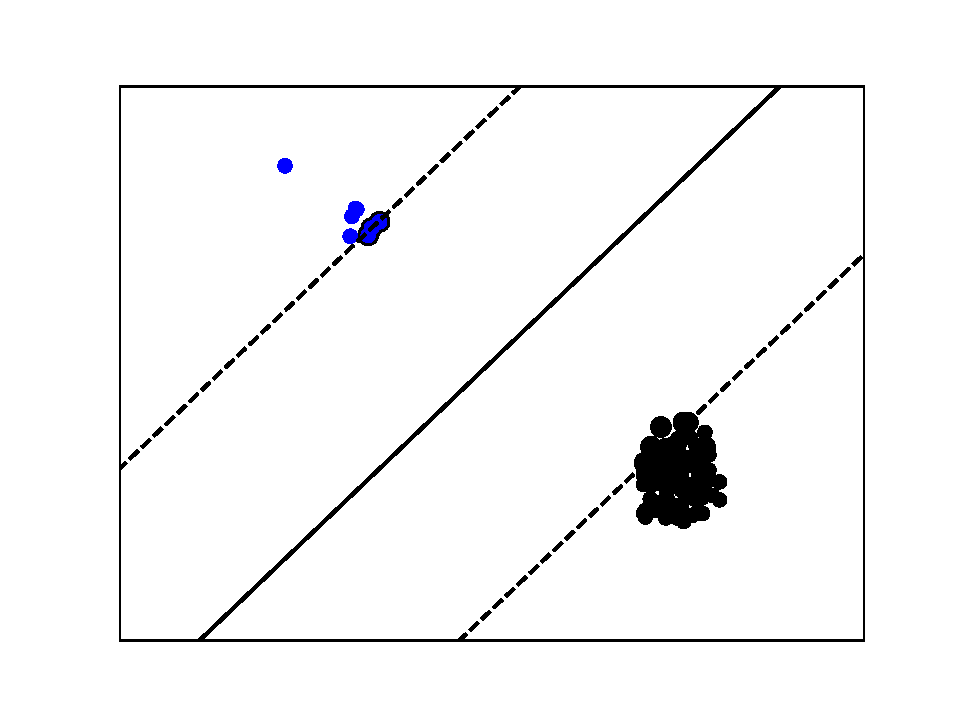
\includegraphics[width=0.7\textwidth]{images/fitC1.pdf} 
        \caption{Classification par SVM à noyau linéaire pour C=1}
    \label{fig:fitC1}
\end{figure}

Sur la figure \ref{fig:fitC1} la frontière de décision sépare correctement les deux classes et se situe globalement à égale distance des groupes de points. La séparation reste équilibrée et la classe minoritaire est encore bien prise en compte.

\begin{figure}[H] 
    \centering
    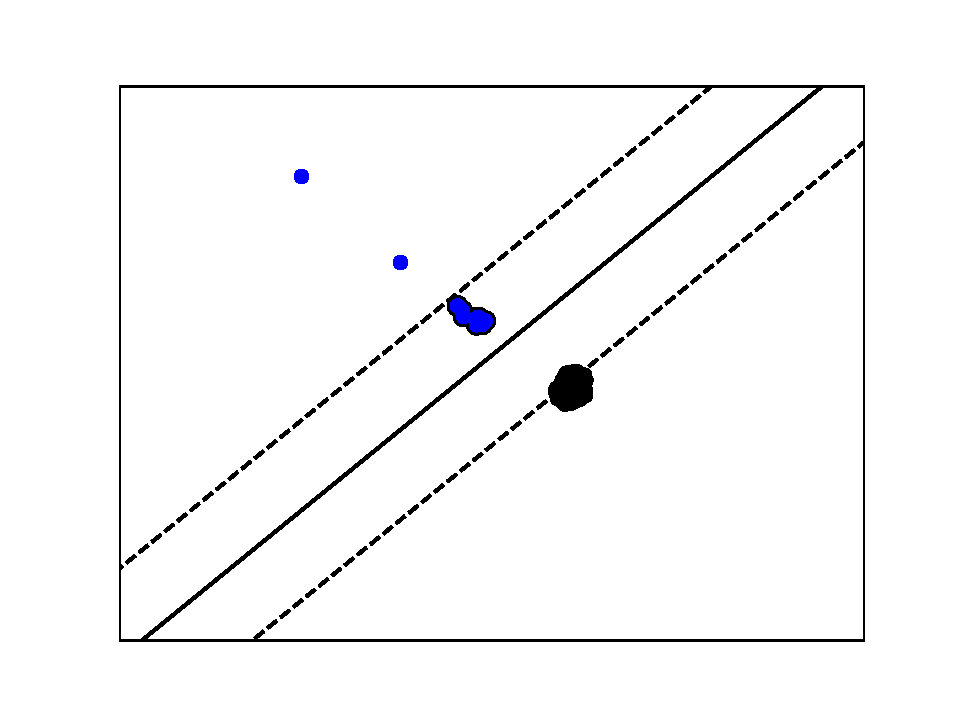
\includegraphics[width=0.7\textwidth]{images/fitC01.pdf} 
    \caption{Classification par SVM à noyau linéaire pour C=0.1}
    \label{fig:fitC01}
\end{figure}

Lorsque l’on diminue $C$ à $0.1$, comme illustré sur la figure \ref{fig:fitC01}, la frontière se déplace progressivement vers la classe minoritaire. En effet, un nombre important de points se retrouve dans la marge. Ces points ne sont pas suffisamment éloignés de l’hyperplan pour permettre une bonne classification et entraînent une pénalité.

\begin{figure}[H] 
    \centering
    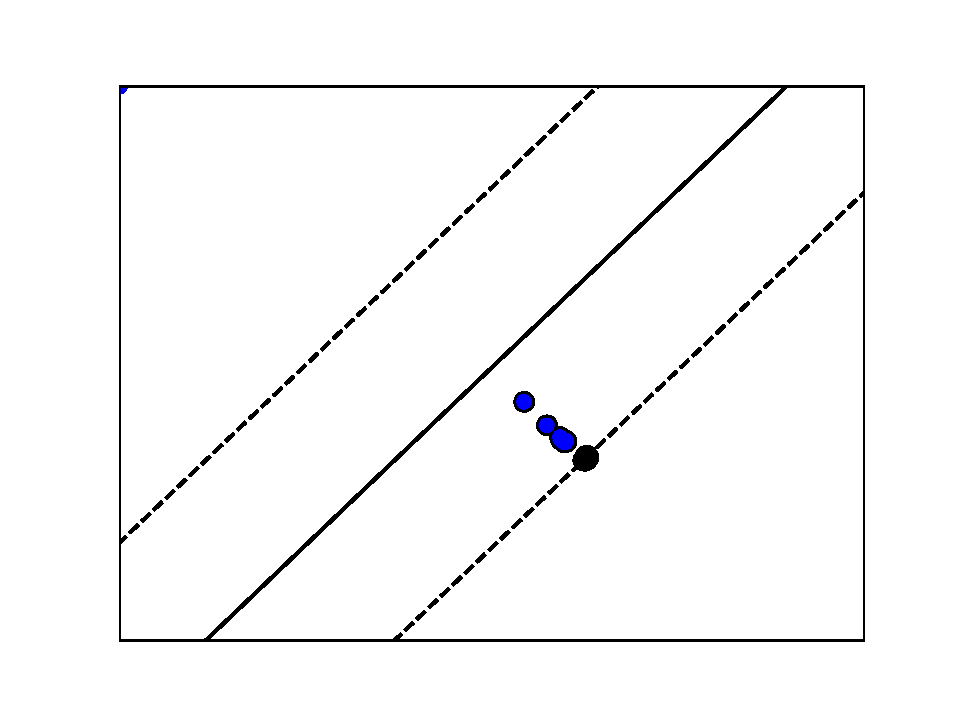
\includegraphics[width=0.7\textwidth]{images/fitC001.pdf} 
    \caption{Classification par SVM à noyau linéaire pour C=0.01}
    \label{fig:fitC001}
\end{figure}

Enfin, en réduisant encore $C$ à $0.01$, la figure \ref{fig:fitC001} montre que la classe minoritaire est quasiment ignorée. La frontière de décision s’aligne presque exclusivement sur la bonne classification de la classe majoritaire, au détriment complet de la minorité.\\

Ainsi, dans le cas d’un dataset très déséquilibré, la diminution de $C$ entraîne systématiquement un déplacement de la frontière de décision vers la classe minoritaire, renforçant le biais en faveur de la classe majoritaire.\\

En pratique, il peut être corrigé en pondérant davantage les erreurs sur la classe minoritaire à l’aide du paramètre class\_weight="balanced" de la classe SVC. Une autre solution consiste à recalibrer les probabilités (probability=True) ou encore à recourir à des techniques de rééchantillonnage (oversampling de la minorité ou undersampling de la majorité).

\section{Classification de visages}

Nous nous intéressons à présent à la problématique de la classification des visages. Nous utilisons ici un jeu de données qui est un extrait prétraité de "Labeled Faces in the Wild" (LFW). Dans ce rapport, nous avons entraîné notre modèle sur deux visages, ceux de Tony Blair et de Colin Powell. Une version équivalente, réalisée sur deux autres visages (Donald Rumsfeld et Colin Powell) est présentée en annexe.

\subsection{Impact du paramètre de régularisation}

Afin d’analyser l’impact du paramètre de régularisation, nous étudions la variation de l’erreur de prédiction en fonction de la valeur de $C$, représentée sur une échelle logarithmique comprise entre $10^{-5}$ et $10^{5}$.


\begin{minted}[frame=single, linenos, fontsize=\small, breaklines]{python}
for C in Cs:
    clf = SVC(kernel='linear', C=C)
    clf.fit(X_train, y_train)   
    scores.append(clf.score(X_train, y_train))
\end{minted}

\begin{minted}[frame=single, fontsize=\small, breaklines]
--- Linear kernel ---
Fitting the classifier to the training set
Best C: 0.001
Best score: 1.0
\end{minted}

Nous obtenons une valeur optimale $C = 0.001$, associée à un score de $1$ sur l’échantillon d’apprentissage. Ce résultat suggère que le modèle est parvenu à séparer parfaitement les données d’entraînement. \\
    
\begin{figure}[H] 
    \centering
    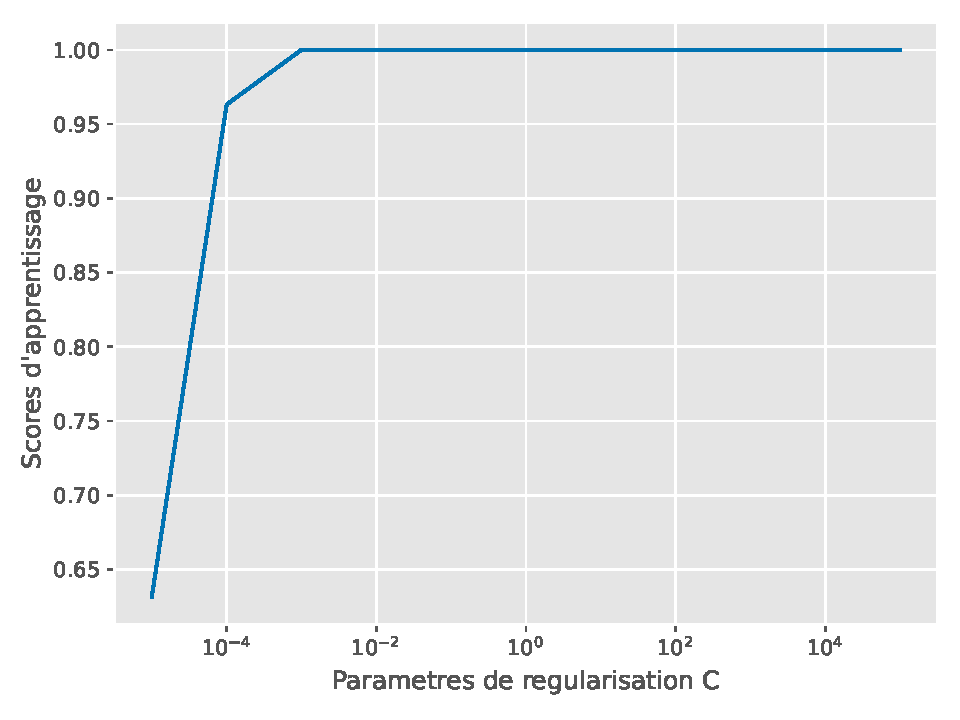
\includegraphics[width=0.7\textwidth]{images/c_score.pdf} 
    \caption{Score d'apprentissage en fonction du paramètre de régularisation $C$}
    \label{fig:c_score}
\end{figure}

La figure \ref{fig:c_score} montre que l’augmentation de $C$ améliore le score d’apprentissage. En revanche, un choix trop élevé de $C$ pourrait amener le modèle à trop bien s’ajuster aux données d’entraînement, au détriment de sa capacité de généralisation, on risque un phénomène de sur-apprentissage.\\

Nous utilisons désormais un SVM à noyau linéaire avec le paramètre C optimal sur notre jeu de données.

\begin{minted}[frame=single, linenos, fontsize=\small, breaklines]{python}
clf = SVC(kernel='linear', C=Cs[ind])
clf.fit(X_train, y_train)
y_pred =clf.predict(X_test)
\end{minted}

Nous obtenons le résultat suivant:

\begin{minted}[frame=single, fontsize=\small, breaklines]
Predicting the people names on the testing set
done in 0.344s
Chance level : 0.6210526315789474
Accuracy : 0.9052631578947369
\end{minted}

Pour évaluer la performance de notre SVM à noyau linéaire sur le jeu de visages, nous la comparons à un niveau de hasard. La proportion d’images correctement classées au hasard est de 62,1\%, ce qui correspond au niveau de chance. En utilisant le paramètre de régularisation optimal $C$, le SVM linéaire atteint une précision de 90,5\% sur le jeu de test, représentant une amélioration significative par rapport au hasard.

\begin{figure}[H] 
    \centering
    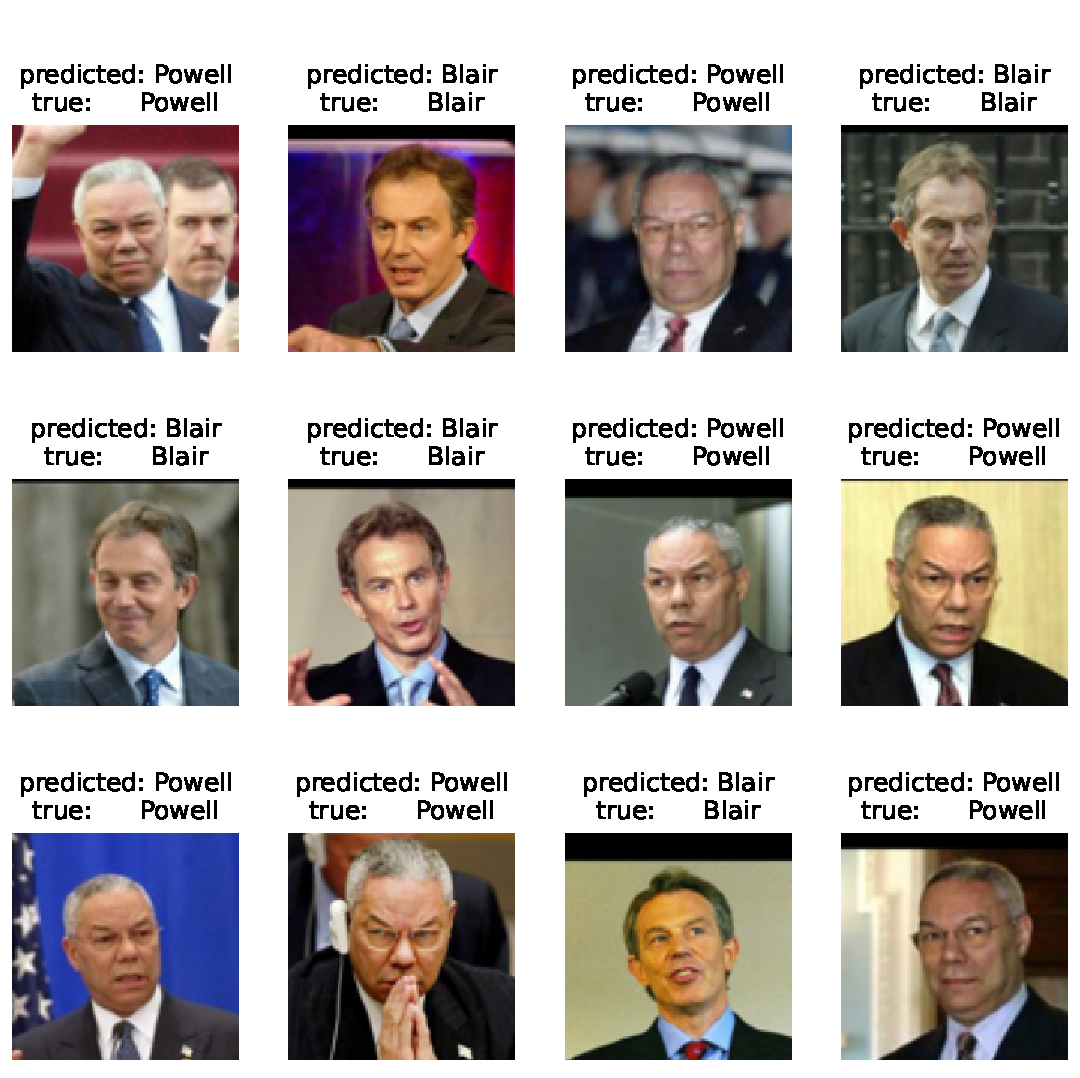
\includegraphics[width=0.7\textwidth]{images/predict_true.pdf} 
    \caption{Comparaison des résultats d’un SVM linéaire avec $C$ optimal}
    \label{fig:predict_true}
\end{figure}

La figure \ref{fig:predict_true} présente un extrait des prédictions de notre modèle pour la reconnaissance faciale. On constate que sur ce petit échantillon, le modèle a parfaitement classé les images.

\begin{figure}[H] 
    \centering
    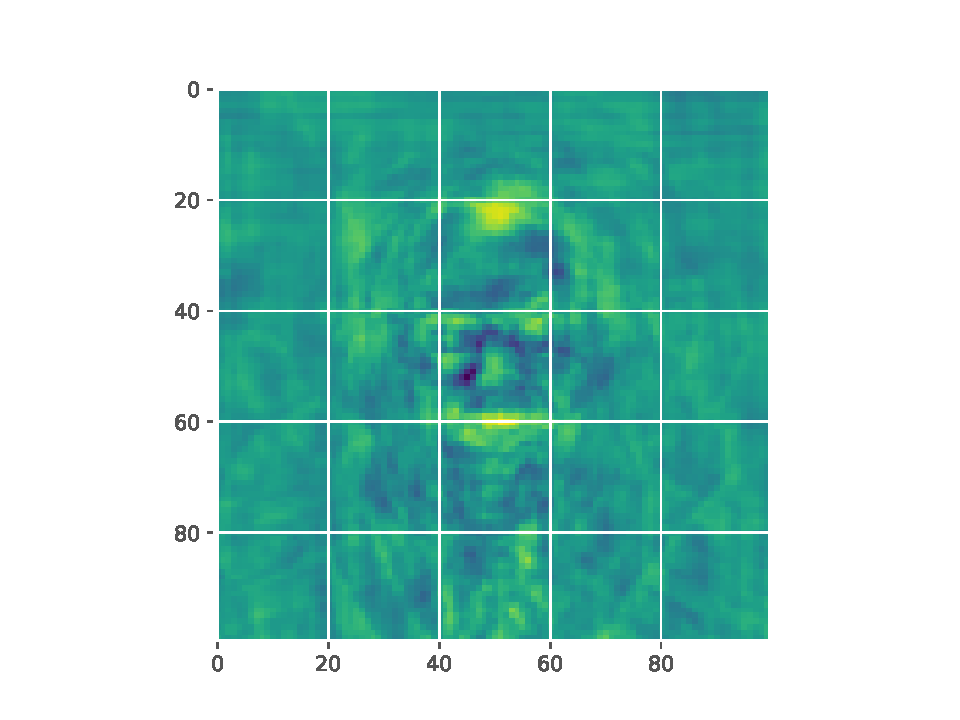
\includegraphics[width=0.7\textwidth]{images/coeffs.pdf} 
    \caption{Visualisation des coefficients}
    \label{fig:coeffs}
\end{figure}

De plus, la figure \ref{fig:coeffs} illustre que le modèle parvient à repérer les traits distinctifs des visages, en accordant un poids particulièrement élevé aux coefficients associés aux yeux, à la bouche et aux cheveux.\\
 
Ainsi, le classificateur est capable de distinguer efficacement les deux individus à partir des caractéristiques extraites des images, et qu’il généralise correctement à de nouvelles données. Le choix de $C$ optimal a permis un compromis efficace entre sous-apprentissage et sur-apprentissage.

\subsection{Introduction de variables de nuisances}

Afin d’étudier la robustesse de notre modèle, nous ajoutons maintenant du bruit aux données d’entrée. 
Plus précisément, nous générons des variables de bruit suivant une distribution gaussienne de moyenne nulle et de variance égale à 1, 
que nous concaténons aux caractéristiques initiales. 

\begin{minted}[frame=single, fontsize=\small, breaklines]{python}
# On rajoute des variables de nuisances
sigma = 1
noise = sigma * np.random.randn(n_samples, 300, ) 
#with gaussian coefficients of std sigma
X_noisy = np.concatenate((X, noise), axis=1)
X_noisy = X_noisy[np.random.permutation(X.shape[0])]
\end{minted}

Nous trouvons les résultats suivants.

\begin{minted}[frame=single, fontsize=\small, breaklines]
Score sans variable de nuisance
Generalization score for linear kernel: 1.0, 0.9105263157894737 

Score avec variable de nuisance
Generalization score for linear kernel: 1.0, 0.48947368421052634
\end{minted}

On observe que malgré un nombre d'échantillons d'apprentissage identique, l'ajout de variables 
bruitées entraîne une chute du score de généralisation de $0,91$ à $0,49$. 
Cela illustre clairement que l'augmentation du nombre de variables, lorsqu'elles ne sont pas pertinentes, 
diminue la capacité du modèle à généraliser correctement.

\subsection{Réduction de dimension}

Afin d’améliorer la capacité de généralisation du classifieur, nous appliquons une réduction de dimension par Analyse en Composantes Principales, ce qui permet de projeter les données dans un sous-espace de plus petite dimension tout en conservant de l’information.

\begin{minted}[frame=single, fontsize=\small, breaklines]
n_components = 120 
pca = PCA(n_components=n_components).fit(X_noisy)
X_bruit = pca.transform(X_noisy)    
run_svm_cv(X_bruit,y)
\end{minted}

Nous avons choisi de mettre en place une boucle faisant varier le nombre de composantes principales retenues lors de la réduction de dimension par ACP. L’objectif est d’observer l’influence de cette réduction progressive sur les performances du classifieur SVM, à la fois sur l’échantillon d’apprentissage et sur l’échantillon de test.

\begin{figure}[H] 
    \centering
    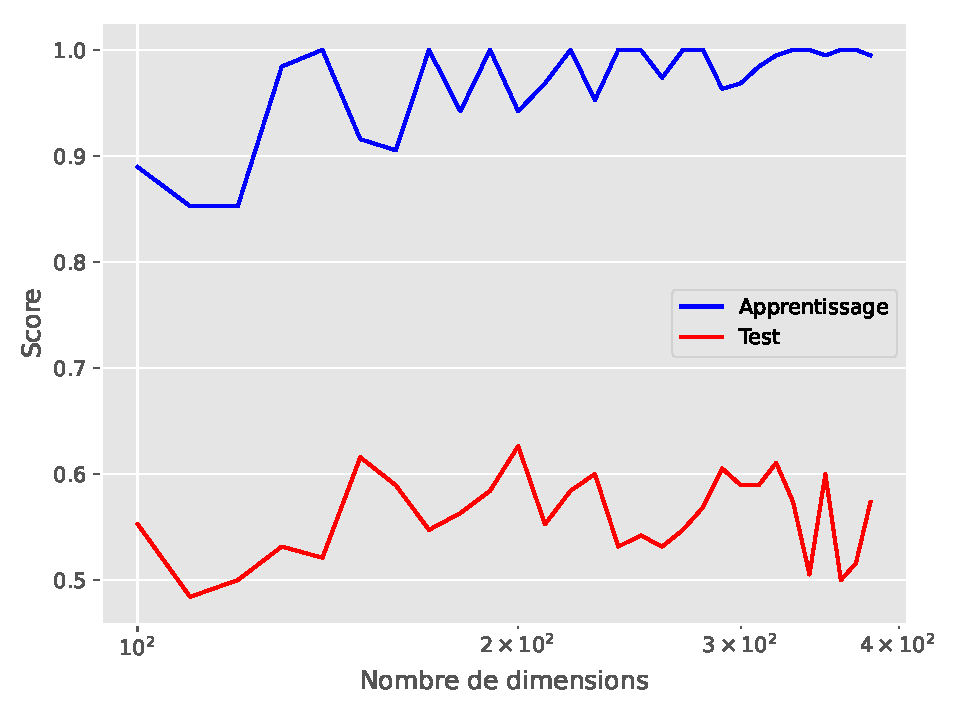
\includegraphics[width=0.7\textwidth]{images/plot_score_train_test.pdf} 
    \caption{Influence de la réduction de dimensions sur les scores}
    \label{fig:ACP}
\end{figure}

Ces résultats montrent que l’augmentation du nombre de dimensions retenues par l’ACP n'améliore pas considérablement le score de test. On observe donc un compromis, conserver trop de dimensions favorise le sur-apprentissage, tandis qu’une réduction trop forte risque de dégrader la représentation des données.

\subsection{Biais dans le pré-traitement}

Dans notre prétraitement des données, un biais se situe au niveau de la conversion des images couleur en niveaux de gris.

\begin{minted}[frame=single, fontsize=\small, breaklines]{python}
X = (np.mean(images, axis=3)).reshape(n_samples, -1)
\end{minted}

En moyennant les trois canaux de couleur, nous perdons toute information liée à la couleur. Or, certaines personnes peuvent être mieux identifiables grâce à des caractéristiques dûes aux couleurs comme la teinte de peau, les cheveux, les vêtements et l'éclairage. Cette transformation peut donc introduire un biais d’information : le modèle ne peut plus exploiter certains indices potentiellement discriminants et pourrait être moins performant pour certaines images ou individus.
Ainsi, la conversion en niveaux de gris simplifie le modèle mais modifie la représentation originale des données, ce qui constitue un biais dans le prétraitement.

\section{Annexe}

\subsection{Classification de visages (Donald Rumsfeld, Colin Powell)}

Afin d’analyser l’impact du paramètre de régularisation, nous étudions la variation de l’erreur de prédiction en fonction de la valeur de $C$, représentée sur une échelle logarithmique comprise entre $10^{-5}$ et $10^{5}$.


\begin{minted}[frame=single, linenos, fontsize=\small, breaklines]{python}
for C in Cs:
    clf = SVC(kernel='linear', C=C)
    clf.fit(X_train, y_train)   
    scores.append(clf.score(X_train, y_train))
\end{minted}

\begin{minted}[frame=single, fontsize=\small, breaklines]
--- Linear kernel ---
Fitting the classifier to the training set
Best C: 0.001
Best score: 1.0
\end{minted}

Nous obtenons une valeur optimale $C = 0.001$, associée à un score de $1$ sur l’échantillon d’apprentissage. Ce résultat suggère que le modèle est parvenu à séparer parfaitement les données d’entraînement. \\
    
\begin{figure}[H] 
    \centering
    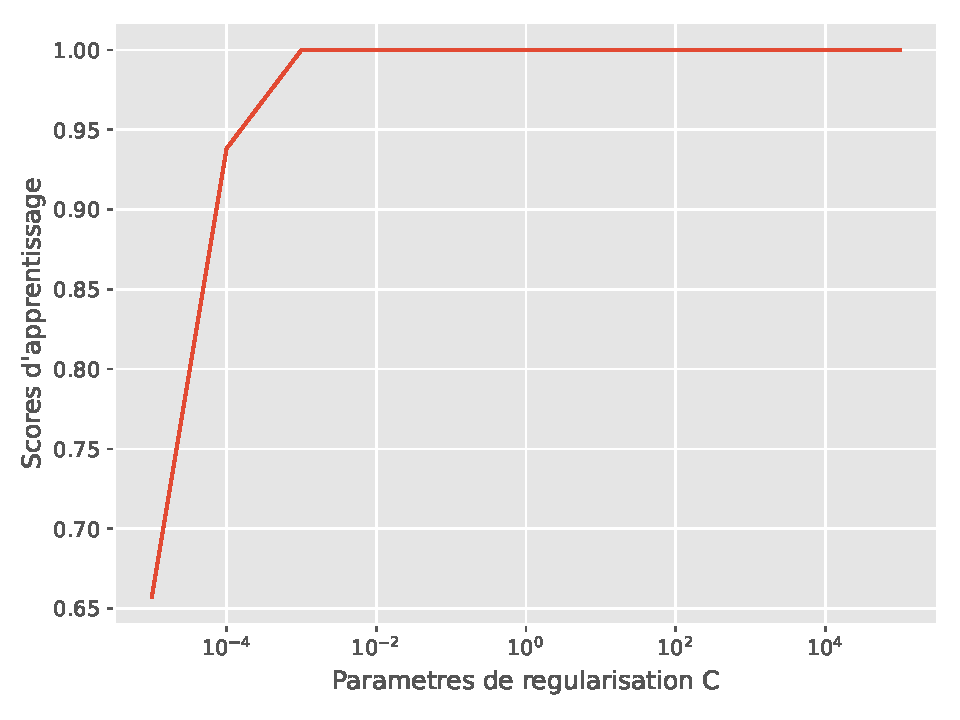
\includegraphics[width=0.7\textwidth]{images/plot_C_annexe.pdf} 
    \caption{Score d'apprentissage en fonction du paramètre de régularisation $C$}
    \label{fig:c_score_ann}
\end{figure}

La figure \ref{fig:c_score_ann} montre que l’augmentation de $C$ améliore le score d’apprentissage. En revanche, un choix trop élevé de $C$ pourrait amener le modèle à trop bien s’ajuster aux données d’entraînement, au détriment de sa capacité de généralisation, on risque un phénomène de sur-apprentissage.\\

Nous utilisons désormais un SVM à noyau linéaire avec le paramètre C optimal sur notre jeu de données.

\begin{minted}[frame=single, linenos, fontsize=\small, breaklines]{python}
clf = SVC(kernel='linear', C=Cs[ind])
clf.fit(X_train, y_train)
y_pred =clf.predict(X_test)
\end{minted}

Nous obtenons le résultat suivant:

\begin{minted}[frame=single, fontsize=\small, breaklines]
Predicting the people names on the testing set
done in 0.203s
Chance level : 0.6610644257703081
Accuracy : 0.8938547486033519
\end{minted}

Pour évaluer la performance de notre SVM à noyau linéaire sur le jeu de visages, nous la comparons à un niveau de hasard. La proportion d’images correctement classées au hasard est de 66,1\%, ce qui correspond au niveau de chance. En utilisant le paramètre de régularisation optimal $C$, le SVM linéaire atteint une précision de 89,3\% sur le jeu de test, représentant une amélioration significative par rapport au hasard.\\ 

\begin{figure}[H] 
    \centering
    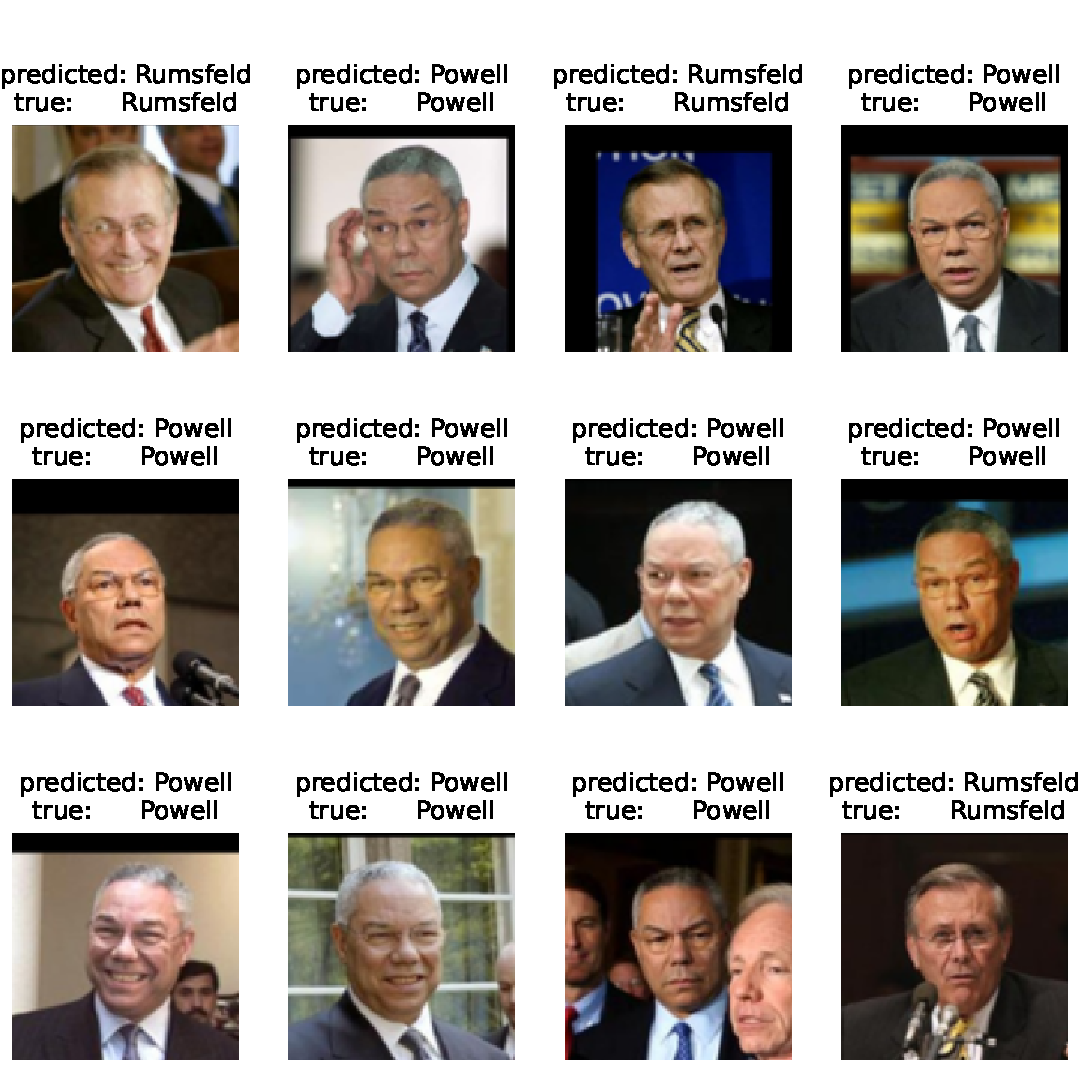
\includegraphics[width=0.7\textwidth]{images/predict_true_annexe.pdf} 
    \caption{Comparaison des résultats d’un SVM linéaire avec $C$ optimal}
    \label{fig:predict_true_ann}
\end{figure}

La figure \ref{fig:predict_true_ann} présente un extrait des prédictions de notre modèle pour la reconnaissance faciale. On constate que sur ce petit échantillon, le modèle a parfaitement classé les images.

\begin{figure}[H] 
    \centering
    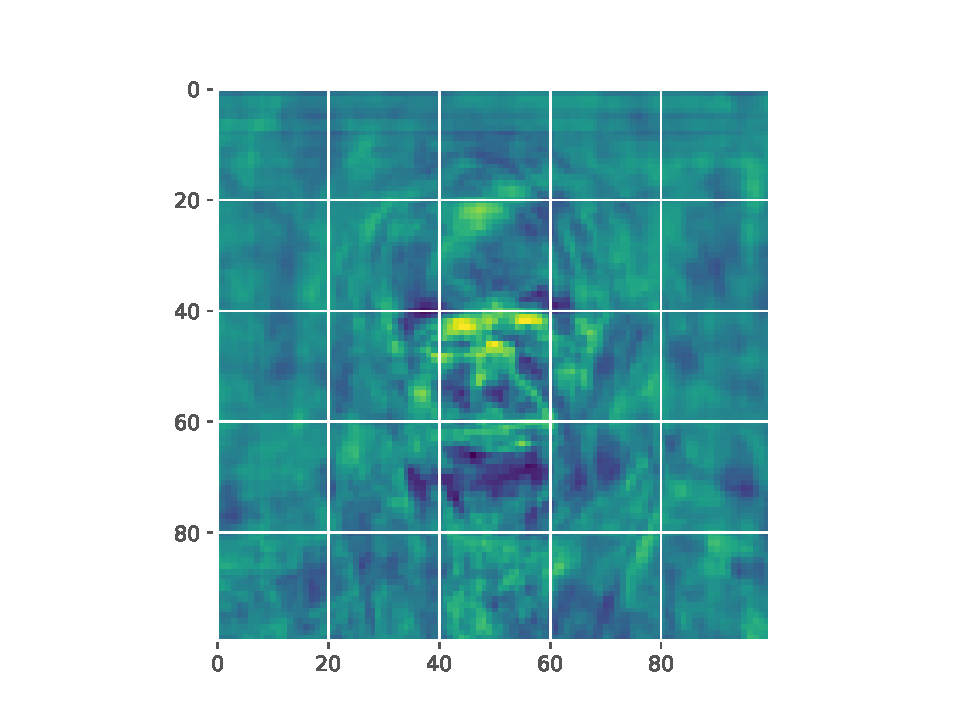
\includegraphics[width=0.7\textwidth]{images/coeffs_annexe.pdf} 
    \caption{Visualisation des coefficients}
    \label{fig:coeffs_annexe}
\end{figure}

De plus, la figure \ref{fig:coeffs_annexe} illustre que le modèle parvient à repérer les traits distinctifs des visages, en accordant un poids particulièrement élevé aux coefficients associés aux yeux, à la bouche et aux cheveux. Dans cette nouvelle étude, le modèle semble également distinguer les lunettes.\\
 
Ainsi, le classificateur est capable de distinguer efficacement les deux individus à partir des caractéristiques extraites des images, et qu’il généralise correctement à de nouvelles données. Le choix de $C$ optimal a permis un compromis efficace entre sous-apprentissage et sur-apprentissage.


\end{document}